
\chapter{Hardware Implementation design space exploration with the Polyhedral Model}
\label{chap:hw_dse:intro}

Based on the conclusion derived from \autoref{chap:dataflow_dse:intro},
the ideal conv. accelerator operates in two modes, direct Mode where 3x3 kernel
with stride 1 are supported and GEMM mode where all other kernel sizes and
strides are supported in GEMM mode via the approach in (REFERENCE LOWERING/
LIFTING CHAPTER). In this section we will deduce the optimal hardware
implementation for the weight stationary dataflow chosen in
\autoref{chap:dataflow_dse:intro} by analyzing data reuse in the loop based
representation of the aforementioned dataflow. To perform this deduction we will
use the polyhedral model to analyse temporal reuse in
\autoref{chap:hw_dse:temporal_analysis} and spatial reuse in
\autoref{chap:hw_dse:spatial_reuse_analysis}. Finally, in
\autoref{chap:hw_dse:simplifying_hierarchy} a simplification of the IFmap memory
hierarchy present in the optimal hardware implementation derived in
\autoref{chap:hw_dse:temporal_analysis} and
\autoref{chap:hw_dse:spatial_reuse_analysis} is presented.

\section{Temporal Reuse Analysis}
\label{chap:hw_dse:temporal_analysis}

Unrolling convolution dataflow loops yield multiple instances of the \ac{MAC}
statement present in the original convolution nested loops in
\autoref{lst:conv_loop}. These instances will be referred to as \ac{MAC} spatial
instances to distinguish them from temporal instances discussed in this chapter.
\ac{MAC} spatial instances can be distinguished based on the memory access
offsets that exist in them as a result of unrolling filter, channel and kernel
loops. For unroll factors F\_T for filters, C\_T for channels, KY\_T and KX\_T
for kernels each statement will have a coresponding access offset based on the
spatial instance index $j \in [0, F\_T*C\_T*KY\_T*KX\_T]$ for each of the data
elements (IFmap, OFmap and Weights) accessed in the loop body. Each \ac{MAC}
spatial instance at index j is characterized by a set of access offsets {Fj, Cj,
KYj, KXj} used by the memory accesses in the \ac{MAC} statement. Applying the
unroll factors and distinguishing each \ac{MAC} statement based on it's
statement index j yields the loop configuration in
\autoref{lst:conv_loops_unrolled}. 

\begin{lstlisting}[language=C, caption=Fully unrolled convolution dataflow loops, label={lst:conv_loops_unrolled}]
    for(int f = 0; f < F; f+=F_T) // Filter loop
        for(int c = 0; c < C; c+=C_T) // Channel loop
            for (int y = 0; y < Y; y++) // FeatureMap Height
                for(int x = 0; x < X; x++) // FeatureMap Width
                        ...
                        /* For all j in [0, F_T*C_T*KY_T*KX_T[ */ 
                        O[f+Fj][y][x] += W[f+Fj][c+Cj][KYj][KXj]* \
                                            I[c][y+KYj][x+KXj] 
                        ...
\end{lstlisting}

Temporal reuse analysis is performed on the above loops. The different
operational modes (GEMM/ Direct) are analysed concurrently using the same loop
representation below as they only differ based on whether we fuse feature map
height and width loops, and set upper bounds of the kernel loops to 1. Since
kernel loops are always unrolled fully this sets KY\_T and KX\_T to 1. We can
analyse temporal reuse in the dataflow represented in
\autoref{lst:conv_loops_unrolled} by adapting the approach in \cite{meeus} 
to the afformentioned dataflow iteration domain and access functions.
Given iteration domain restrictions imposed by the polyhedral model,
\autoref{lst:poly:analysis} assumes unroll factors F\_T =
C\_T = 4. Setting F\_T and C\_T to concrete values does not affect output
results of temporal reuse analysis.

\clearpage
\begin{lstlisting}[caption=Polyhedral analysis of reuse in iscc for convolution loops, label={lst:poly:analysis}]
    // Define iteration domain for all accessed data elements
    ID:=[F, C, Y, X] -> { S[f, c, y, x] : 0<=f<F and 0<=c<C and f mod 4=0 and c mod 4=0, 0<=y<Y and 0<=x<X};
    // Define access functions for each data element
    IFMAP:=([Cj, KYj, KXj] -> {S[f, c, y, x] -> IF[c+Cj][y+KYj][x+KXj]})*ID;
    OFMAP:=([Fj] -> {S[f, c, y, x] -> PS[f+Fj][y][x]})*ID;
    WEIGHT:=([Fj, Cj, KYj, KXj] -> {S[f, c, y, x] -> W[f+Fj][c+Cj][KYj][KXj]})*ID;
    // Evaluate temporal reuse
    IFMAP_REUSE:=(IFMAP.(IFMAP^-1))*(ID<<ID);
    OFMAP_REUSE:=(OFMAP.(OFMAP^-1))*(ID<<ID);
    WEIGHT_REUSE:=(WEIGHT.(WEIGHT^-1))*(ID<<ID);  

\end{lstlisting}

In \autoref{lst:poly:analysis}, the iteration domain for the loops in
\autoref{lst:conv_loops_unrolled} is converted into it's set representation in
line 2 where for some access statement S the loop iteration vector [f, c, y, x,]
is bound by the upper and lower bounds [0, F], [0, C], [0, Y], [0, X]
respectively. These bounds are represented by the associated parameters passed
to the iteration domain set assignment in line 2. Each memory accessed in the
body of the loop has an access function at each level of that memory's
hierarchy. As a result, each instance of the loop iteration vector [f, c, y, x]
is mapped to a memory access for each of the memories in lines 4-6. Access
offsets used in the memory access functions are passed as parameters based on
the convention established in \autoref{lst:conv_loops_unrolled}. This mapping
creates multiple temporal instances for each memory access in each \ac{MAC}
spatial instance.  For
example, for some iteration vector [f = 1, c = 1, y = 0, x = 1],
 the OFmap access that occurs at iteration vector [f = 2, c= 1, y = 0,
x = 1] is a different temporal instance of the same OFmap access at [f = 1, c = 1,
y = 0, x = 1]. 
Two accesses that access the same index but at different
iteration vectors are different temporal instances of the same access.
After applying the operation in lines 8-10, we can determine the
temporal reuse behavior of the accessed memories in the convolution loops.  
\autoref{lst:poly:result} shows the reuse behavior for each memory. Original
iteration domains constraints are ommited for brevity. 

\clearpage
\begin{lstlisting}[caption=Polyhedral analysis results w.r.t data elements in convolution loops, label={lst:poly:result}]
    IFMAP_REUSE;
    [F, C, Y, X, Cj, KYj, KXj]->{
        S[f, c, y, x] -> S[f', c' = c, y' = y, x' = x] :
            ... f' > f and 0 <= f' < F ... 
        }
    OFMAP_REUSE;
    [F, C, Y, X, Fj]->{ 
        S[f, c, y, x] -> S[f' = f, c', y' = y, x' = x] : 
            ... c' > c and 0 <= c' < C ... 
        }
    WEIGHT_REUSE;
    [F, C, Y, X, Fj, Cj, KYj, KXj] -> { 
        S[f, c, y, x] -> S[f' = f, c' = c, y', x'] : 
            ... y' > y and 0 <= y' < Y and 0 <= x' < X ...; 
    }
\end{lstlisting}

\autoref{lst:poly:result} shows the temporal reuse behavior in memory accesses. For each
of the memories accessed (IFmap, OFmap and Weights) there exists a set of reuse
(IFMAP\_REUSE, OFMAP\_REUSE and WEIGHT\_REUSE) maps that map each iteration
vector of an access to all the proceeding iteration vectors where that same
access occurs. From the above listing we can see that, in the set of IFmap reuse
maps (IFMAP\_REUSE), IFmap channels are reused temporally with respect to filter
loops. For a given IFmap accessed at channel c, that channel is accessed again
when computing the output for all proceeding filter loop iterationtions f' where
$f'>f$. The absence of other mappings in the set of reuse maps IFMAP\_REUSE shows
that 1) this reuse behavior holds at any arbitrary iteration vector [f, c, y, x]
and 2) this reuse behavior depends only on the filter loop. For the set OFmap
reuse maps (OFMAP\_REUSE), for an OFmap acceess at iteration vector [f, c, y,
x], it is accessed again at loop iteration f'=f, c', y'=y, x'=x where $c'>c$.  
For (WEIGHT\_REUSE) Weights exhibit temporal reuse w.r.t feature map width and
height, the X and Y loops. 

Applying the hardware taxonomy in \cite{maestro}, IFmap exhibits temporal reuse,
multicast communication. OFmap exhibits temporal reuse, reduction communication
given their read-modify-write behavior. Weights exhibit temporal multicast
communication. Given the limited implementation options derivable from temporal
reuse we can comfortably define the appropriate connectivity and memory
hierarchies for IFmaps channels, OFmaps channels (equivelent to number of
Filters), and Weights. The beginings of a hardware template derived from the
afformentioned temporal reuse behavior of the different memories referenced in
the convolution dataflow can be seen in \ref{fig:reuse_illus}. In
\ref{fig:reuse_illus} the template is broken into 3 major componenets. The first
is the IFmap memory hierarchy currently with only 1 level. The 2nd component is
the compute portion of the template where partial sums are computed and
aggregating into OFmap data elements. Finally the 3rd component which is the
OFmap memory that stores OFmap partial sums until they are aggregated into OFmap
pixels and are written back to memory.

\begin{figure}[]
    \centering
    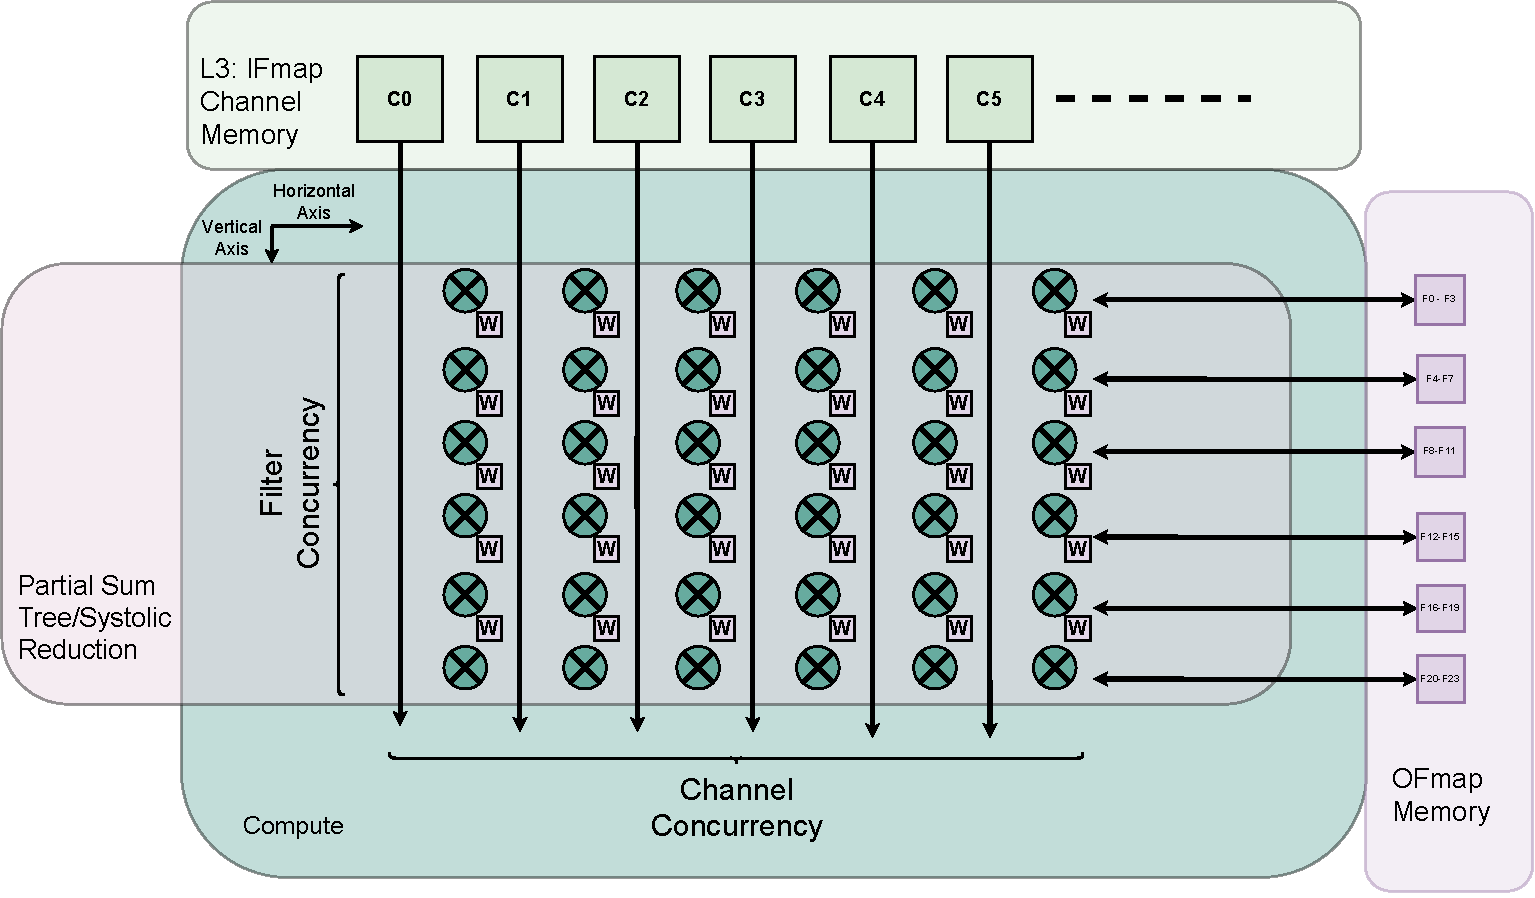
\includegraphics[scale=0.4]{fig/reuse_illus.pdf}
    \caption{Initial hardware template incorporating buffers IFmap and OFmap temporal reuse}
    \label{fig:reuse_illus}
\end{figure}

In addition to the temporal reuse behavior exhibited across IFmap channels,
temporal reuse exists within individual IFmap channels due to the stencil based
access pattern arising from the X, Y, KY, KX loops in the dataflow. That
temporal reuse is affected by the decision to fully unroll kernel loops which
causes temporal reuse to exist between unrolled IFmap kernel ports. Proof of the
existence of that temporal reuse is given in the polyhedral analysis in
\autoref{lst:poly:xy_reuse}. 

\begin{lstlisting}[caption=Analysis of IFmap channel reuse, label={lst:poly:xy_reuse}]
    ID_XY:=[Y, X, KY, KX] -> { S[y, x, ky, kx] : 0<=ky<KY and 0<=kx<KX and 0<=y<Y and 0<=x<X};
    IFMAP_XY:=({S[y, x, ky, kx] -> IF[y+ky][x+kx]})*ID;
    IFMAP_REUSE_XY:=(IFMAP_XY.(IFMAP_XY^-1))*(ID_XY<<ID_XY);
    IFMAP_XY_REUSE;
    [Y, X, KY, KX] -> { 
        S[y, x, ky, kx] -> S[y', x', ky' = (y - y') + ky, kx' = (x - x') + kx] : 
            ... y' > y and (y + ky) -KY < y' <= (y + ky) and (x + kx) -KX < x' <= (x + kx) ...;
    }
\end{lstlisting}

\begin{figure}[]
    \centering
    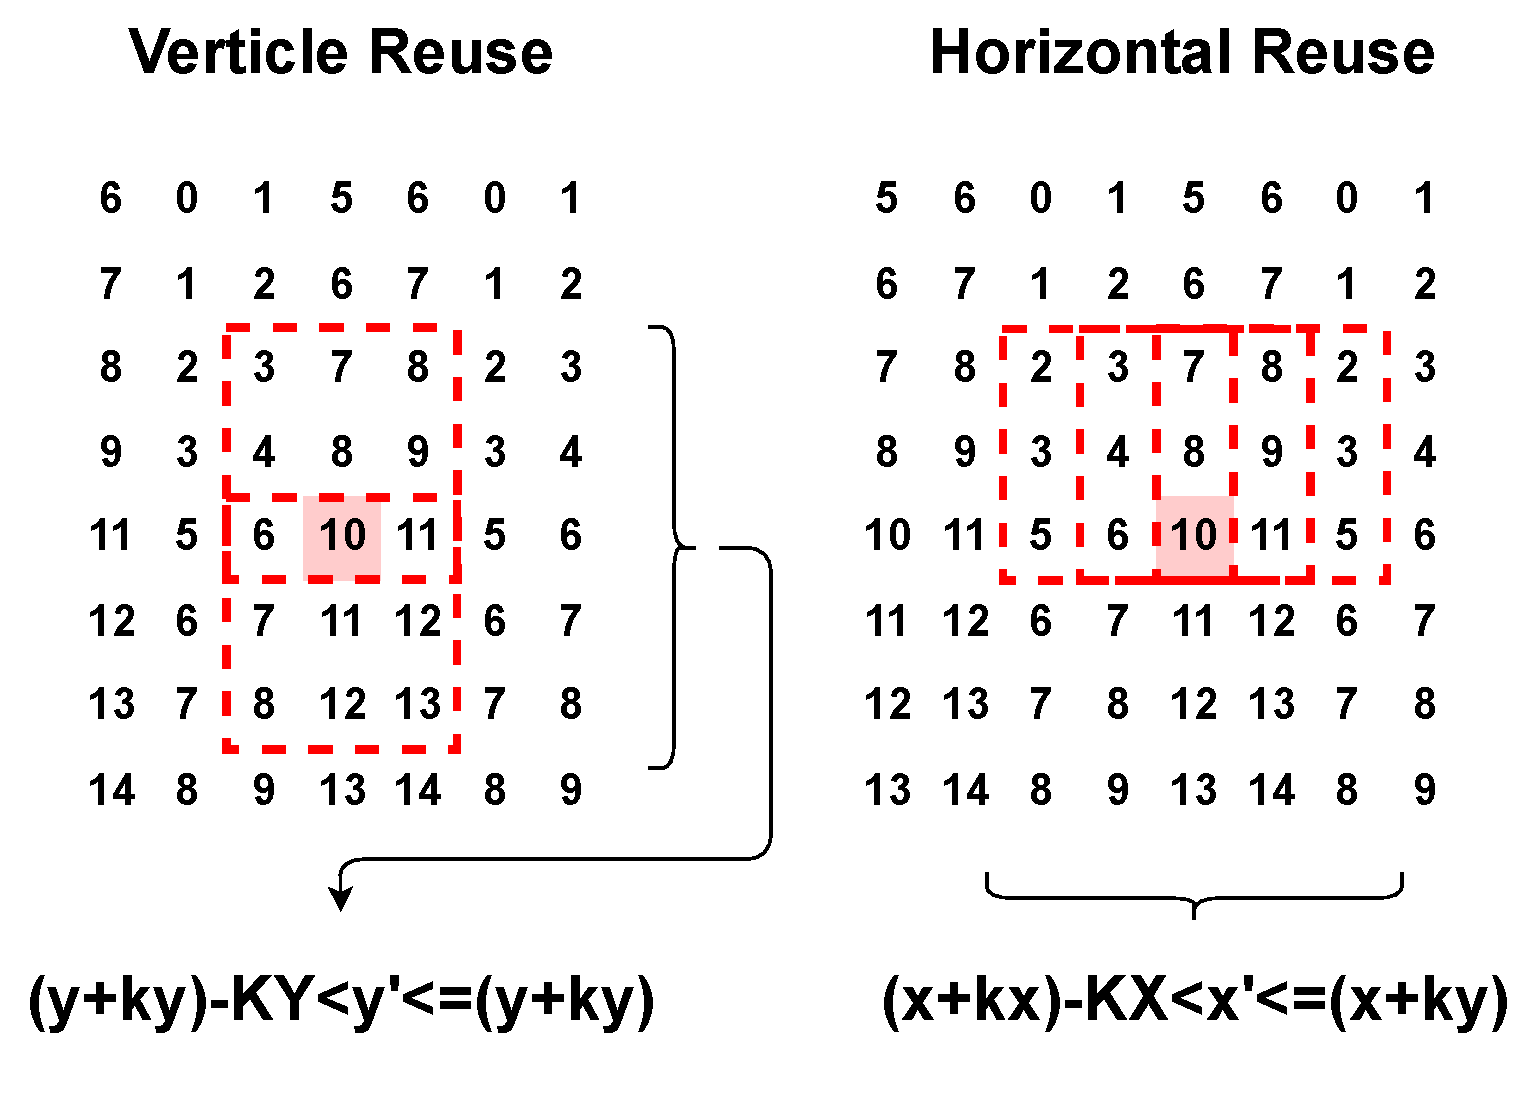
\includegraphics[scale=0.4]{fig/xy_reuse.pdf}
    \caption{IFmap Reuse Behavior w.r.t individual feature map channels}
    \label{fig:ifmap_xy_reuse}
\end{figure}

Within an individual IFmap channel, temporal reuse is exhibited w.r.t X and Y
loops. Given the complexity of the domain constraints of IFMAP\_XY\_REUSE in
\autoref{lst:poly:xy_reuse}, an illustration of the reuse behavior is available
in \figref{fig:ifmap_xy_reuse}. In \figref{fig:ifmap_xy_reuse}, individual
pixels within the kernel are reused based on the position of the sliding window
or stencil of the convolution in an IFmap channel. There are two primary
directions where that reuse is exhibited, vertical and horizontal with an IFmap
channel. The loops that control the verticle and horizontal stencil position in
the IFmap are the Y and X loops in the dataflow. Because kernel loops are fully
unrolled, the temporal reuse exhibited in \autoref{lst:poly:xy_reuse} occurs
accross unrolled kernel loop ports. To determine the appropriate memory
infrastructure to support that stencil based access pattern, we can apply the
technique in \cite{meeus} to construct a reuse chain that moves reused data
between urnolled kernel ports. The advantage of using a reuse chain is that the
temporal reuse that exists within an IFmap channel is relegated to a smaller
memory with lower memory access cost.

\cite{meeus} constructs a reuse chain for applications with a sliding window
access pattern that connects each unrolled kernel port with it's neighbors using
a FIFO or a shift register. If the temporal reuse distances between the accesses
of neighboring ports are constant \cite{meeus} uses a shift register, otherwise
they use a FIFO. The reuse distance between accesses of neighboring ports are
then converted into storage of the same size. So if two ports share the same
data but with a lag of 2 iterations in the iteration domain they're operating
in, then a shift register of size 2 can be placed between them. Similar to the
sliding window application explored in \cite{meeus} the reuse distances between
the unrolled kernel ports in the convolution dataflow are also constant. To
determine the reuse distances necessary between ports we can apply the analysis
in \autoref{lst:poly:xy_buffer_sizing:analysis} adapted from \cite{meeus} to
determine the sizing of the buffers in the reuse chain for IFmap accesses within
a channel. The analysis in \autoref{lst:poly:xy_buffer_sizing:analysis} assumes
a kernel size of 3x3. 


\begin{lstlisting}[caption=Determining buffer sizes in 3x3 convolutions, label={lst:poly:xy_buffer_sizing:analysis}]
    ID:=[IFMAP_Y, IFMAP_X] -> {S[y,x]:y>=0 and x>=0 and y<=IFMAP_Y-3 and x<=IFMAP_X-3};
    A0:=[IFMAP_Y, IFMAP_X] -> {S[y,x]->A[y+0,x+0]}*ID;
    A1:=[IFMAP_Y, IFMAP_X] -> {S[y,x]->A[y+0,x+1]}*ID;
    A2:=[IFMAP_Y, IFMAP_X] -> {S[y,x]->A[y+0,x+2]}*ID;
    A3:=[IFMAP_Y, IFMAP_X] -> {S[y,x]->A[y+1,x+0]}*ID;
    ...
    A8:=[IFMAP_Y, IFMAP_X] -> {S[y,x]->A[y+2,x+2]}*ID;

    R10:=(lexmin ((A1.A0^-1)*(ID<<ID)));
    R21:=(lexmin ((A2.A1^-1)*(ID<<ID)));
    R32:=(lexmin ((A3.A2^-1)*(ID<<ID)));
    ...
    R87:=(lexmin ((A8.A7^-1)*(ID<<ID)));
\end{lstlisting}

In \autoref{lst:poly:xy_buffer_sizing:analysis}, the iteration domain for the YX
loops are defined as functions of the IFmap dimensions passed as parameters (line 1).
The unrolled kernel loop IFmap accesses are then described using access maps
that map the iteration vector [y,x] to the associated IFmap access (lines 2-7).
Notice that the accesses are described as constant offsets added to access iterators y
and x. These constants represent the kernel loop iterators ky, and kx that are now
unrolled. For each neighboring pair of ports accessing the IFmap we can
determine the reuse behavior in (lines 9-10). Operations in lines (9-13) map
iterations where a port accesses a data element in IFmap with the earliest next
iteration in which the neighboring port accesses that same data element. The
distance between the accesses is then used as the reuse buffer size. The results
of the analysis are presented in \autoref{lst:poly:xy_buffer_sizing:results}.

\clearpage 

\begin{lstlisting}[caption=Polyhedral analysis of reuse in iscc for convolution loops, label={lst:poly:xy_buffer_sizing:results}]
R10;
$1 := [IFMAP_Y, IFMAP_X] -> { 
    S[y, x] -> S[y' = y, x' = 1 + x] : 
        0 <= y <= -3 + IFMAP_Y and 0 <= x <= -4 + IFMAP_X 
}
R21;
$2 := [IFMAP_Y, IFMAP_X] -> { 
    S[y, x] -> S[y' = y, x' = 1 + x] : 
        0 <= y <= -3 + IFMAP_Y and 0 <= x <= -4 + IFMAP_X 
}
R32;
$3 := [IFMAP_Y, IFMAP_X] -> { 
    S[y, x] -> S[y' = 1 + y, x' = -2 + x] : 
        0 <= y <= -4 + IFMAP_Y and 2 <= x <= -3 + IFMAP_X 
}
...
R87;
$8 := [IFMAP_Y, IFMAP_X] -> { 
    S[y, x] -> S[y' = y, x' = 1 + x] : 
        0 <= y <= -3 + IFMAP_Y and 0 <= x <= -4 + IFMAP_X 
}
\end{lstlisting}

In \ref{lst:poly:xy_buffer_sizing:results}, reuse distances between neighboring
ports depend on the relationship between the ports and whether their access offsets
are in the same row of the stencil or not. If two neighboring ports have unequal
ky offsets the reuse distance between them is IFMAP\_X-3. If two neighboring
ports have an equal ky offset the reuse distance is 1. An example of the first
case is lines 11-15 where the reuse distance between port 2 and port 3 is
IFmap-3. The evidence of that is that for any data accessed at port 3 with
iteration vector y, x that same data is accessed at port 2 at iteration vector
[y+1, x-2]. Based on the lexicographic ordering of iteration vector [y, x] and [y+1,
x-2], the distance between those two vectors is IFMAP\_X-3, or in terms of OFmap
dimensions X-1. Applying the same analysis to two ports in the same row (R10,
R21, R45, R87, ...) yields a reuse distance of 1 as evidence by the iteration
vectors of access [y, x] and [y, x+1] in all of the afformentioned neighboring
port pairs. 

Applying the results of the analysis in
\autoref{lst:poly:xy_buffer_sizing:results} with the previous template \autoref{fig:reuse_illus}
results in the updated template \autoref{fig:reuse_chain}.

\begin{figure}[]
    \centering
    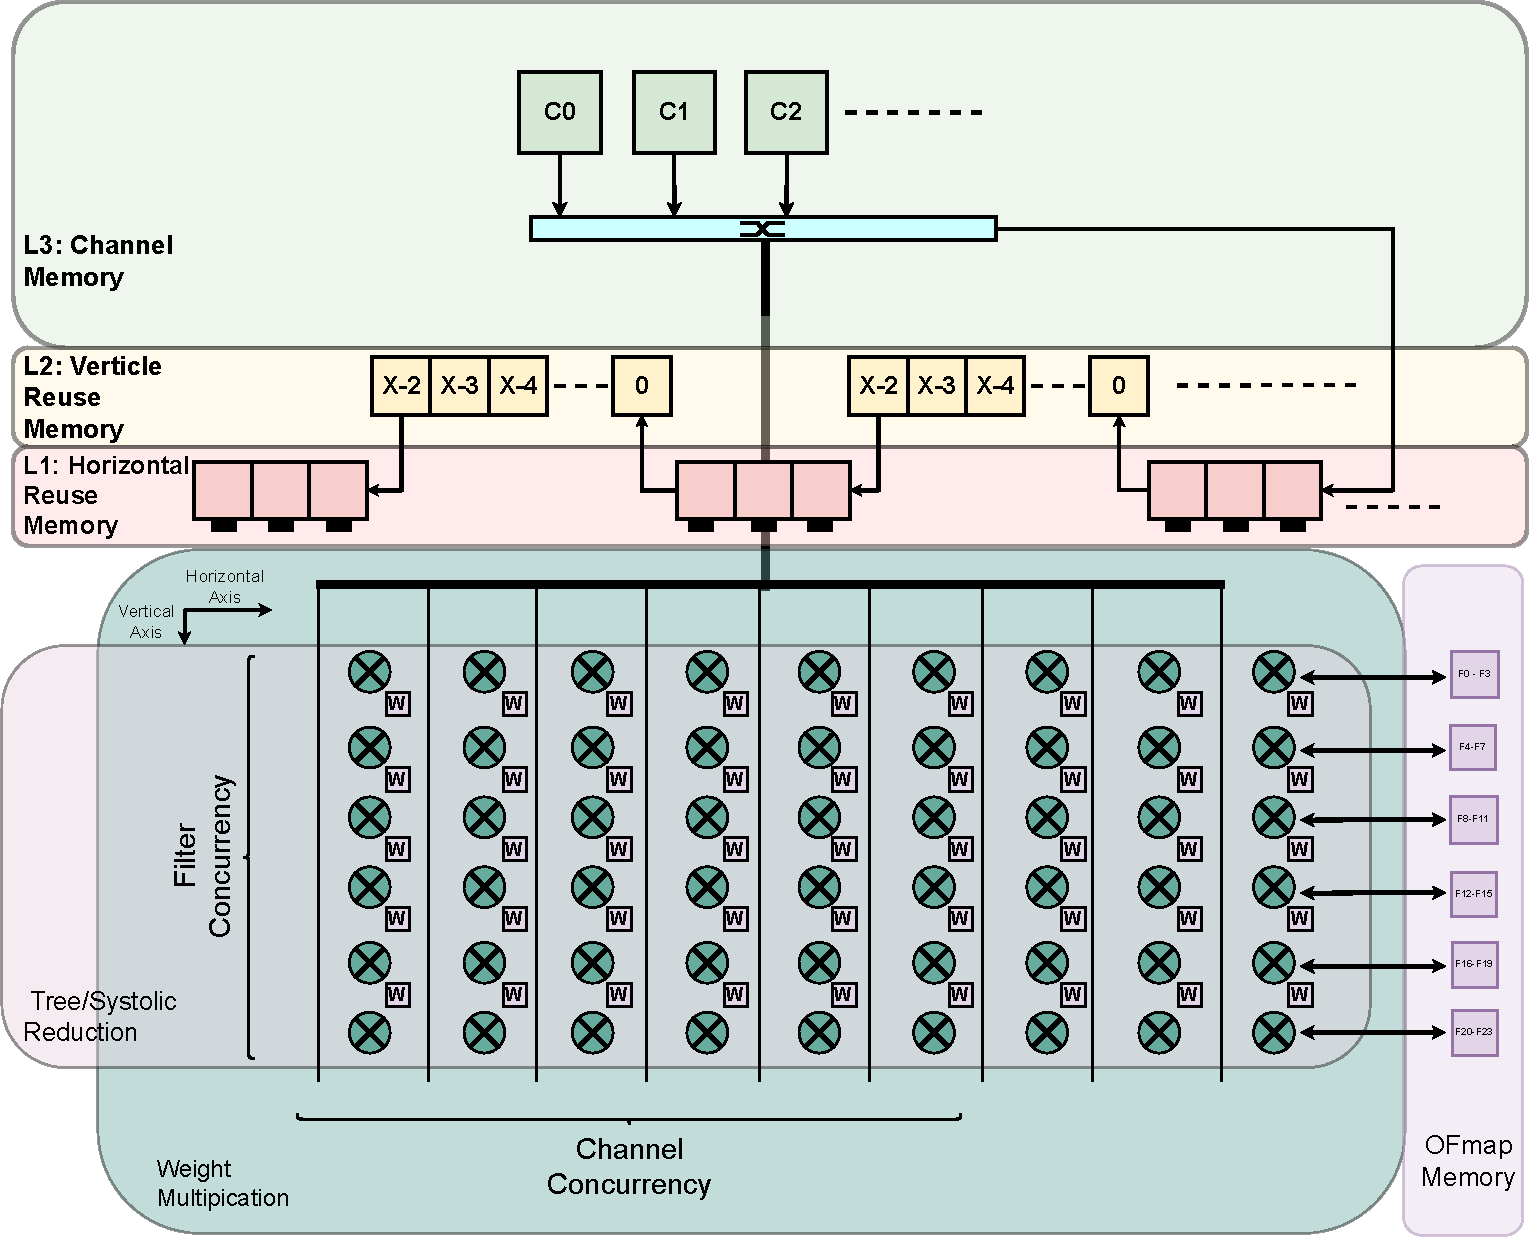
\includegraphics[scale=0.4]{fig/reuse_chain.pdf}
    \caption{Hardware template incorporating a reuse chain for reuse within an IFmap channel }
    \label{fig:reuse_chain}
\end{figure}


\section{Spatial Reuse Analysis}
\label{chap:hw_dse:spatial_reuse_analysis}

So now we know the hierarchy needed to express X and Y reuse in IFmap. Applying
the unroll factors in the target loops in the dataflow will yield a loop
structure similar to the one in \ref{lst:conv_loops_unrolled_fully}. Using the
convention established in \ref{chap:hw_dse:temporal_analysis}, each
\ac{MAC} statement in the unrolled loop body has an associated j index. In the
loop body there exists duplicate memory accesses across individual \ac{MAC}
spatial instances. Those duplicate accesses are highlighted in
\autoref{lst:conv_loops_unrolled_fully} and they are the origin of spatial reuse
in the dataflow. IFmaps exhibit spatial reuse with multicast communication w.r.t
to filter loops. OFmap exhibit spatial reuse with reduction communication
w.r.t to channel loops. Weights exhibit no spatial reuse 
 
\clearpage
\begin{lstlisting}[language=C, caption=Spatial reuse in fully unrolled kernel loops, label={lst:conv_loops_unrolled_fully}]
for(int f = 0; f < F; f+=F_T) // Filter loop
    for(int c = 0; c < C; c+=C_T) // Channel loop
        for (int y = 0; y < Y; y++) // FeatureMap Height
            for(int x = 0; x < X; x++) // FeatureMap Width
            {
                %\colorbox{green}{O[f+0][y][x]}% += W[f+0][c+0][0][0] * \ 
                                    %\colorbox{yellow}{I[c+0][y+0][x+0]}%; // j=0
                %\colorbox{green}{O[f+0][y][x]}% += W[f+0][c+0][0][1] * \
                                    %\colorbox{yellow}{I[c+0][y+0][x+1]}%; // j=1
                %\colorbox{green}{O[f+0][y][x]}% += W[f+0][c+0][0][2] * \
                                    I[c+0][y+0][x+2];  // j=2
                %\colorbox{green}{O[f+0][y][x]}% += W[f+0][c+0][1][0] * \ 
                                    I[c+0][y+1][x+2];  // j=3
                ...
                %\colorbox{red}{O[f+1][y][x]}% += W[f+1][c+0][0][0] * \
                                    %\colorbox{yellow}{I[c+0][y+0][x+0]}%; // j=C_T*KY_T*KX_T
                %\colorbox{red}{O[f+1][y][x]}% += W[f+1][c+1][0][1] * \
                                    %\colorbox{yellow}{I[c+0][y+0][x+1]}%; // j=C_T*KY_T*KX_T+1
                ...
                O[f+F_T-1][y][x] += W[f+F_T-1][c+C_T-1][KY_T-1][KX_T-1] * \ 
                                        I[c][y+KY_T-1][x+KX_T-1]; 
                                                    // j=F_T*C_T*KY_T*KX_T-1
                                        
            }
\end{lstlisting}

Applying the taxonomy in \autoref{fig:hw_taxonomy} to data elements that are
spatially reused, IFmap channels that are spatially reused across unrolled
filter loops can be broadcast with a bus. The reuse chain discussed in
\autoref{chap:hw_dse:temporal_analysis} can be thought of as a
Store\&Forward scheme to deliver individual IFmap channel data elements to the
\ac{PE}s for reduction into OFmaps.Weights reused for channel iteration and are
discarded. They exhibit no spatial reuse, just temporal. Therefore they should
be kept in small on chip buffers, preferably close to the computation they are
used in. OFmap exhibit spatial reuse across concurrent channels as well as
temporal reuse across channel sets as discussed in
\autoref{chap:hw_dse:temporal_analysis}. A reduction tree as in
\autoref{fig:reduction_styles}.a or a systolic array reduce and fwd as in
\autoref{fig:reduction_styles}.b are both possible assuming no restrictions
arising from synthesis. Combining the reuse chain derived in
\autoref{chap:hw_dse:temporal_analysis} with the required systolic
delays yields a simplification to the L1 memory present in
\autoref{fig:reuse_chain}. This simplification is discussed in
\autoref{chap:hw_dse:simplifying_hierarchy}.


\begin{figure}
    \centering
    \subfigure[]{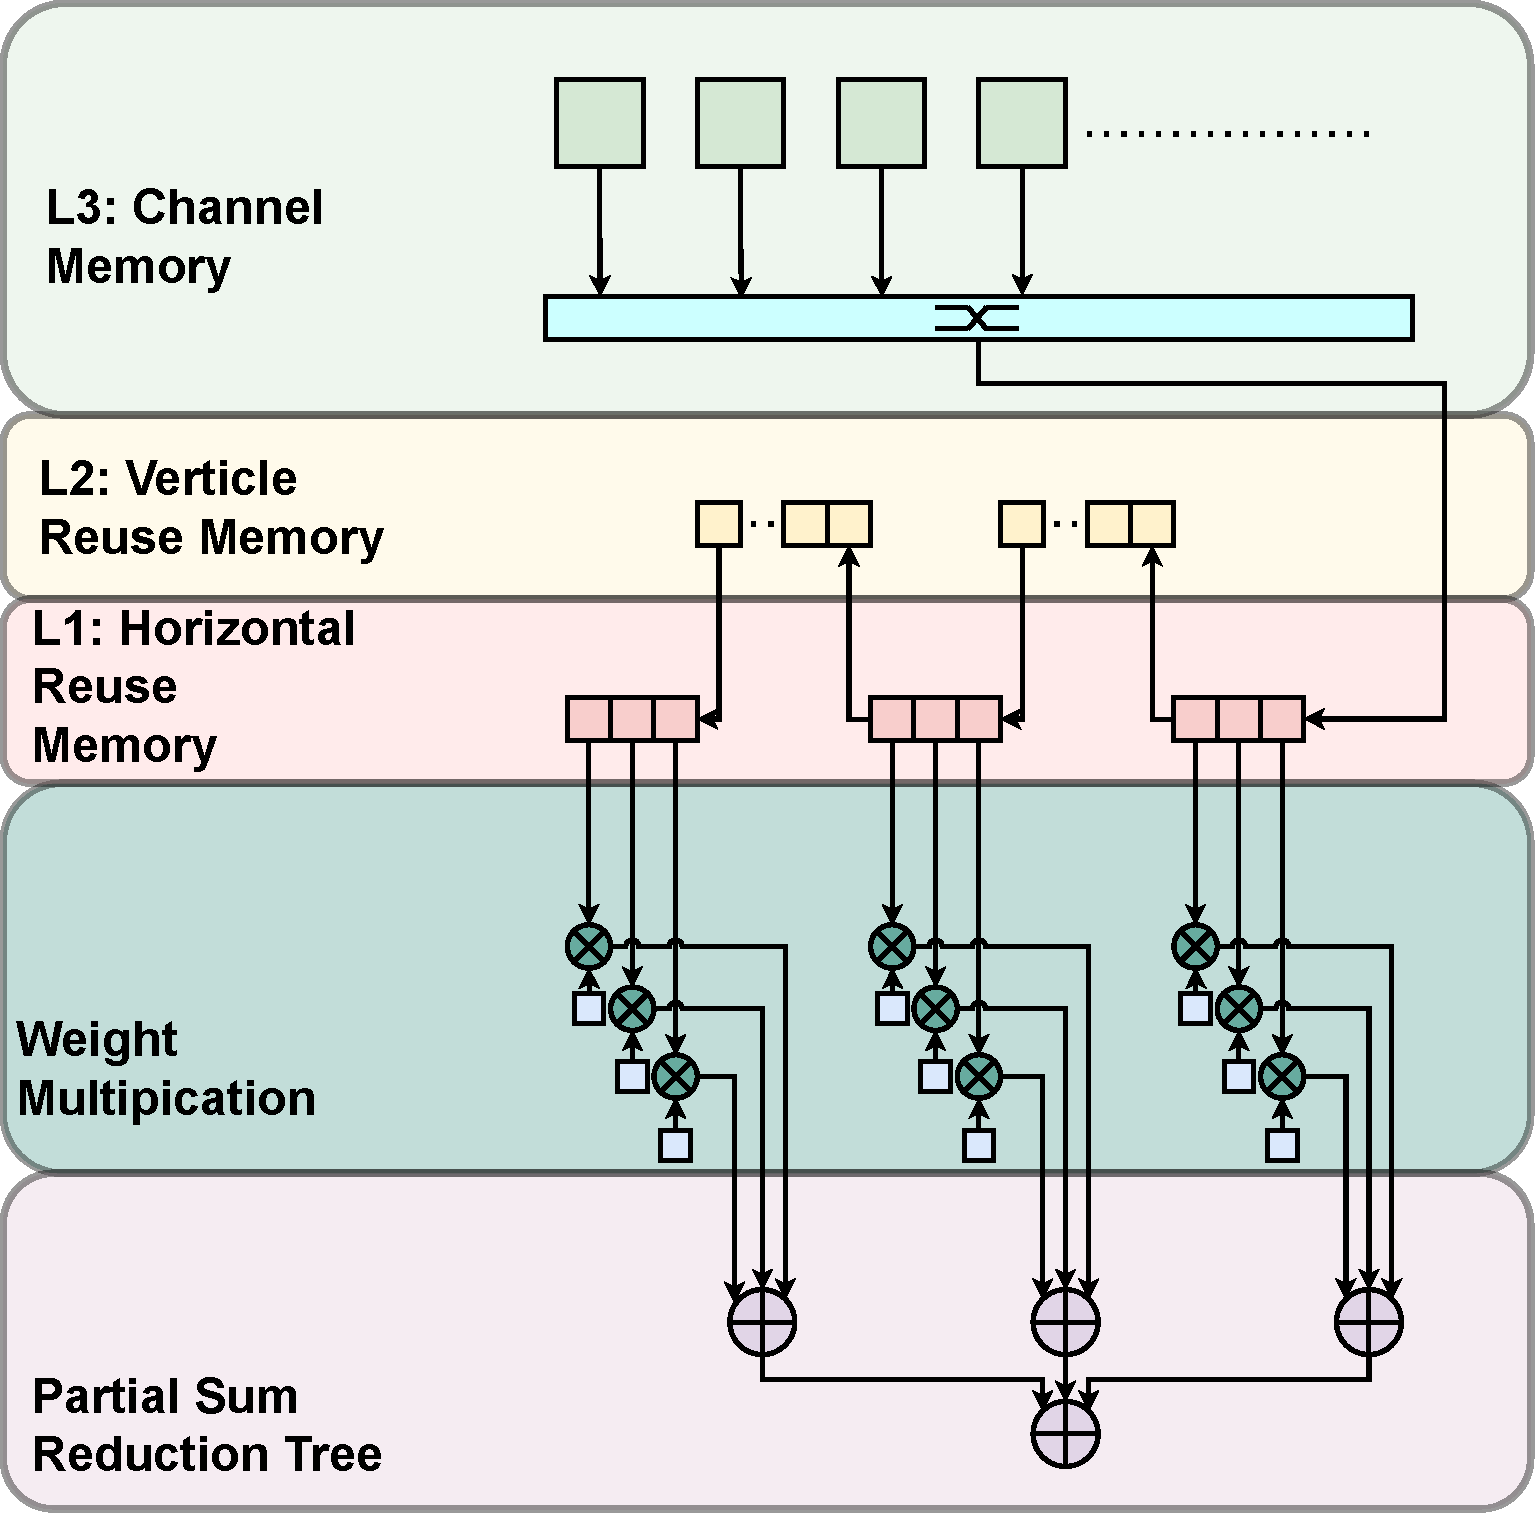
\includegraphics[width=0.5\textwidth]{fig/treeReduction.pdf}}
    \subfigure[]{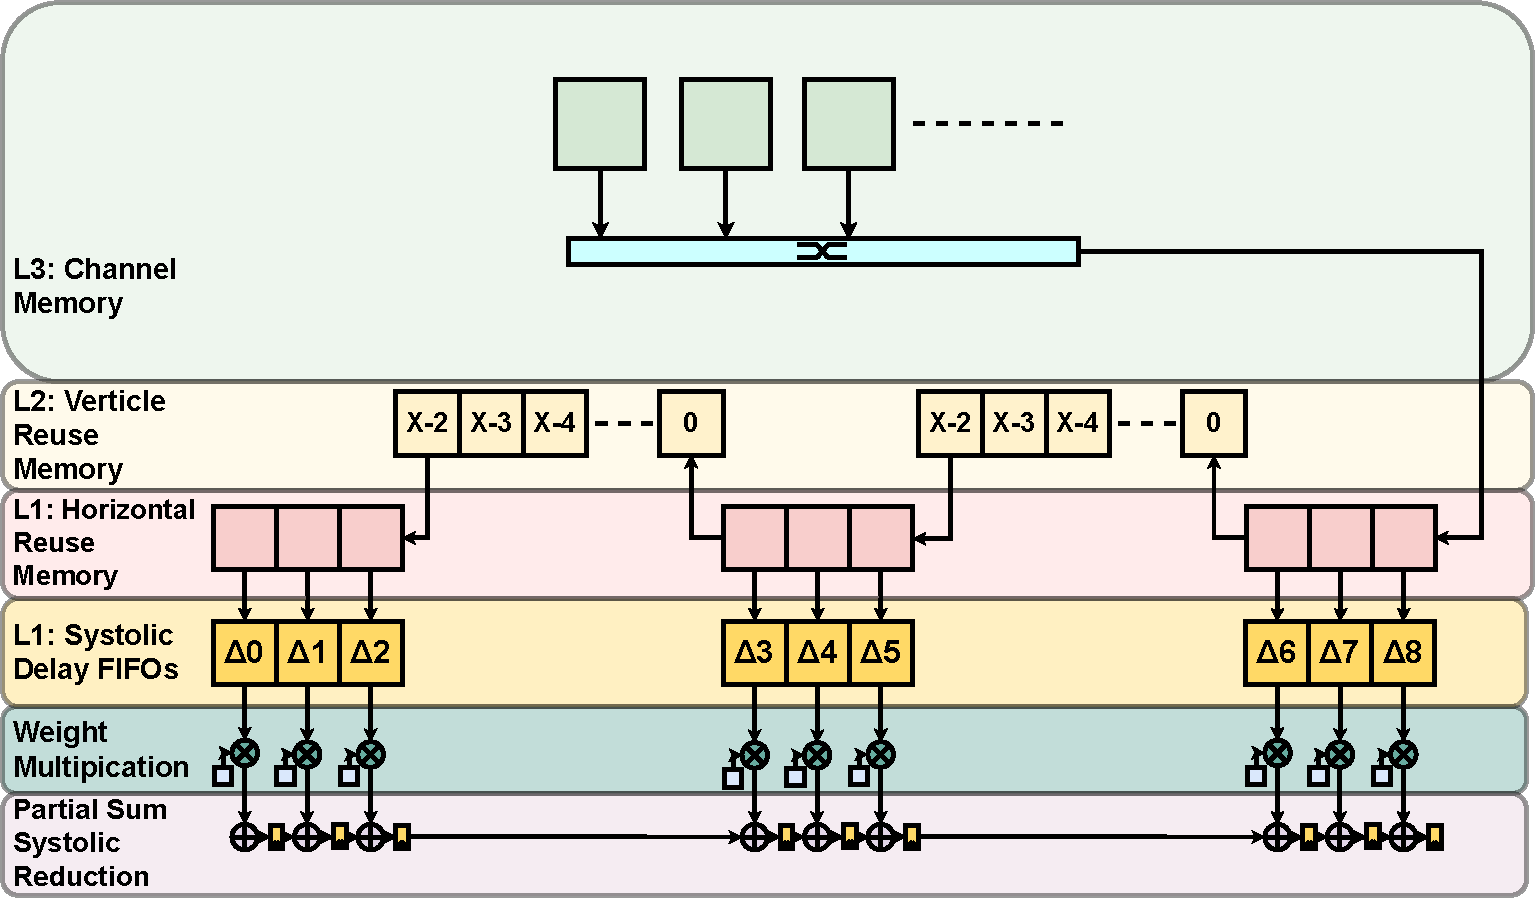
\includegraphics[width=0.7\textwidth]{fig/SystolicReduction.pdf}}
    \caption{Illustration of different partial sum reduction styles assuming kernel size is 3x3 (a) Tree Reduction (b) Systolic array reduction}
    \label{fig:reduction_styles}
\end{figure}

\section{Simplifying the memory hierarchy}
\label{chap:hw_dse:simplifying_hierarchy}

\begin{figure}[]
    \centering
    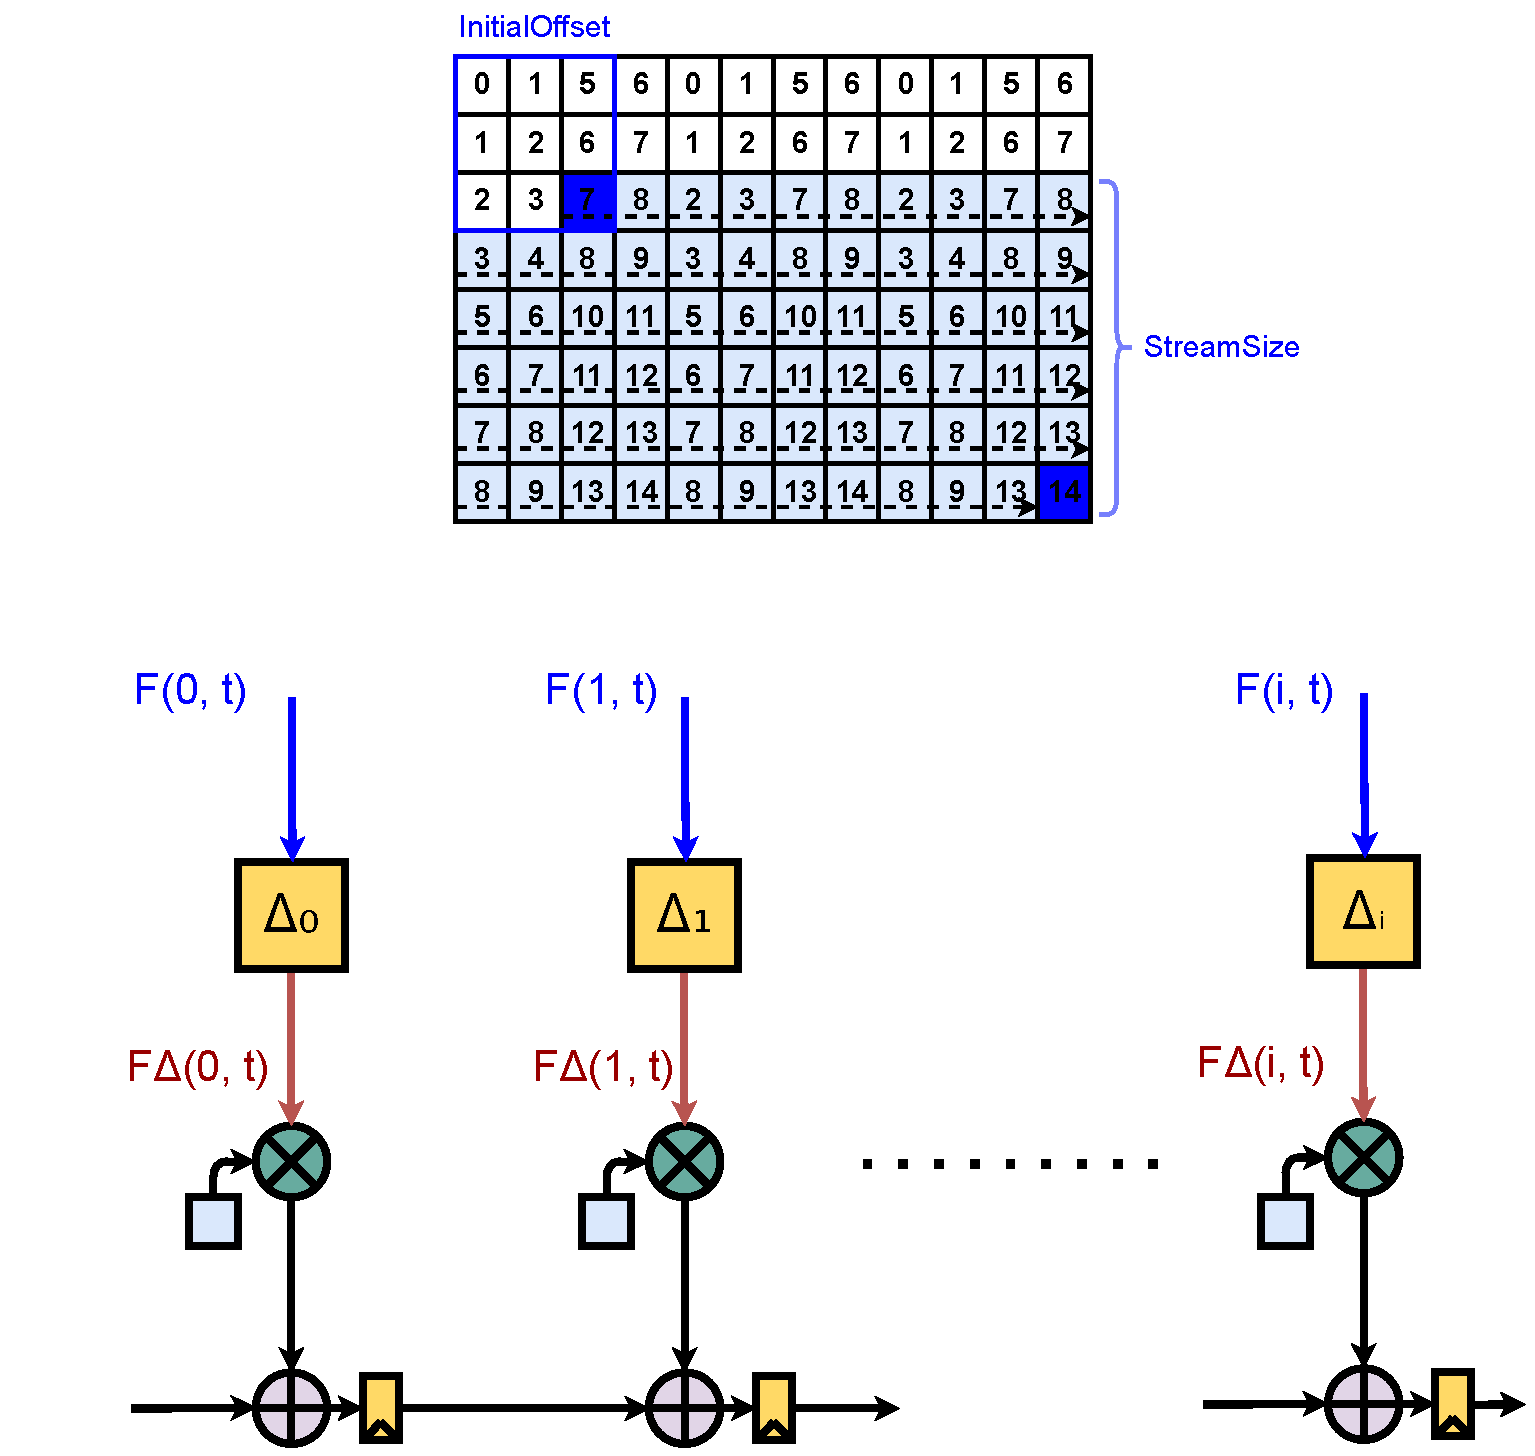
\includegraphics[scale=0.5]{fig/delayproof.pdf}
    \caption{Reinterpretation of IFmap memory hierarchy outputs as a stream function}
    \label{fig:delay_proof}
\end{figure}

We can reinterpret the accesses made by the IFmap memory hierarchy in
\autoref{fig:reuse_chain} as a stream function $F(i, t)$ whose output produces
element from an IFmap channel. The variable $i$ is the port index of IFmap
hierarchy and $t$ is the time in cycles since the beginning of the convolution
operation. A representation of this reinterpretation of the accesses made in the
IFmap memory hierarchy can be seen in \autoref{fig:delay_proof}. Since it's
always assumed that in direct mode kernel loops are unrolled fully the number of
ports into the IFmap memory hierarchy is always a multiple of $K^2$ where $K$ is
the size of the kernel being processed in direct mode. 

\begin{gather}
    IFmap \in R^{C\times n \times n} \xrightarrow{Reshape} IFmap \in R^{1\times Cn^2} \\
    Weight \in R^{F\times C\times K \times K} \\
    F(i, t)=    \begin{cases}
                    IFmap_{A(i, t)} & 0<=t < StreamSize \\
                    0 & else
                \end{cases} \\
    StreamSize = n(n-K)+(n-K) \\
    A(i, t) = InitialOffset(i) + t\\
\end{gather}

Each data element streamed from the IFmap depends on the an access function that
also takes the same variables $i$ and $t$. Depending on the port index $i$ the
access function for each port is composed on an initial offset in the IFmap and
the current cycle count. The number of cycles in which output from the IFmap
memory hierarchy can be produced is limited to the stream size of the IFmap
currently being processed. The stream size is a function of the IFmap dimensions
and the kernel Size. 

\begin{gather}
    InitialOffset = C_in^2+Y_in+X_i \\
    C_i = \lfloor \frac{\lfloor \frac{i}{K} \rfloor}{K} \rfloor \\
    Y_i = (\lfloor \frac{i}{K} \rfloor ) \bmod K\\
    X_i = i \bmod K = (i - \lfloor \frac{i}{K} \rfloor K)\\
\end{gather}

The initial offset function defines the initial index
offset in the IFmap the stream starts from for each port $i$. It can be
decomposed into three main offsets. A channel offset $C_i$, a row offset $Y_i$
and a column offset $X_i$. 

\begin{gather}
    F_\Delta(i, t) = \begin{cases}
    IFmap_{A_\Delta(i, t)} & \Delta_i<=t < \Delta_i+ StreamSize \\
    0 & else
    \end{cases} \\
    \Delta_i = i \\
    A_\Delta(i,t) = A(i, t) - \Delta_i\\
    % \hat{OFmap}(j) = \displaystyle\sum\limits_{i=0}^{ub(i)} A_\Delta(i, j+i)
\end{gather}

Under this new streaming based interpretation of the accesses in the IFmap
memory hierarchy, the delay elements in the systolic reduction scheme in
\autoref{fig:reduction_styles}.b are represented as time shifts in the stream
function $F(i,t)$. These time shifts are represented in the new delayed access
function $A_\Delta(i, t)$.

\begin{gather}
    A_\Delta(i,t) =  C_in^2+Y_in+(i - \lfloor \frac{i}{K} \rfloor K) + t- i\\
    A_\Delta(i,t) =  \lfloor \frac{\lfloor \frac{i}{K} \rfloor}{K} \rfloor^2+(\lfloor \frac{i}{K} \rfloor ) \bmod K + \underbrace{(- \lfloor \frac{i}{K} \rfloor K)}_{X'_i} + t\\
    % \hat{OFmap}(j) = \displaystyle\sum\limits_{i=0}^{ub(i)} A_\Delta(i, j+i)
\end{gather}

\begin{figure}[]
    \centering
    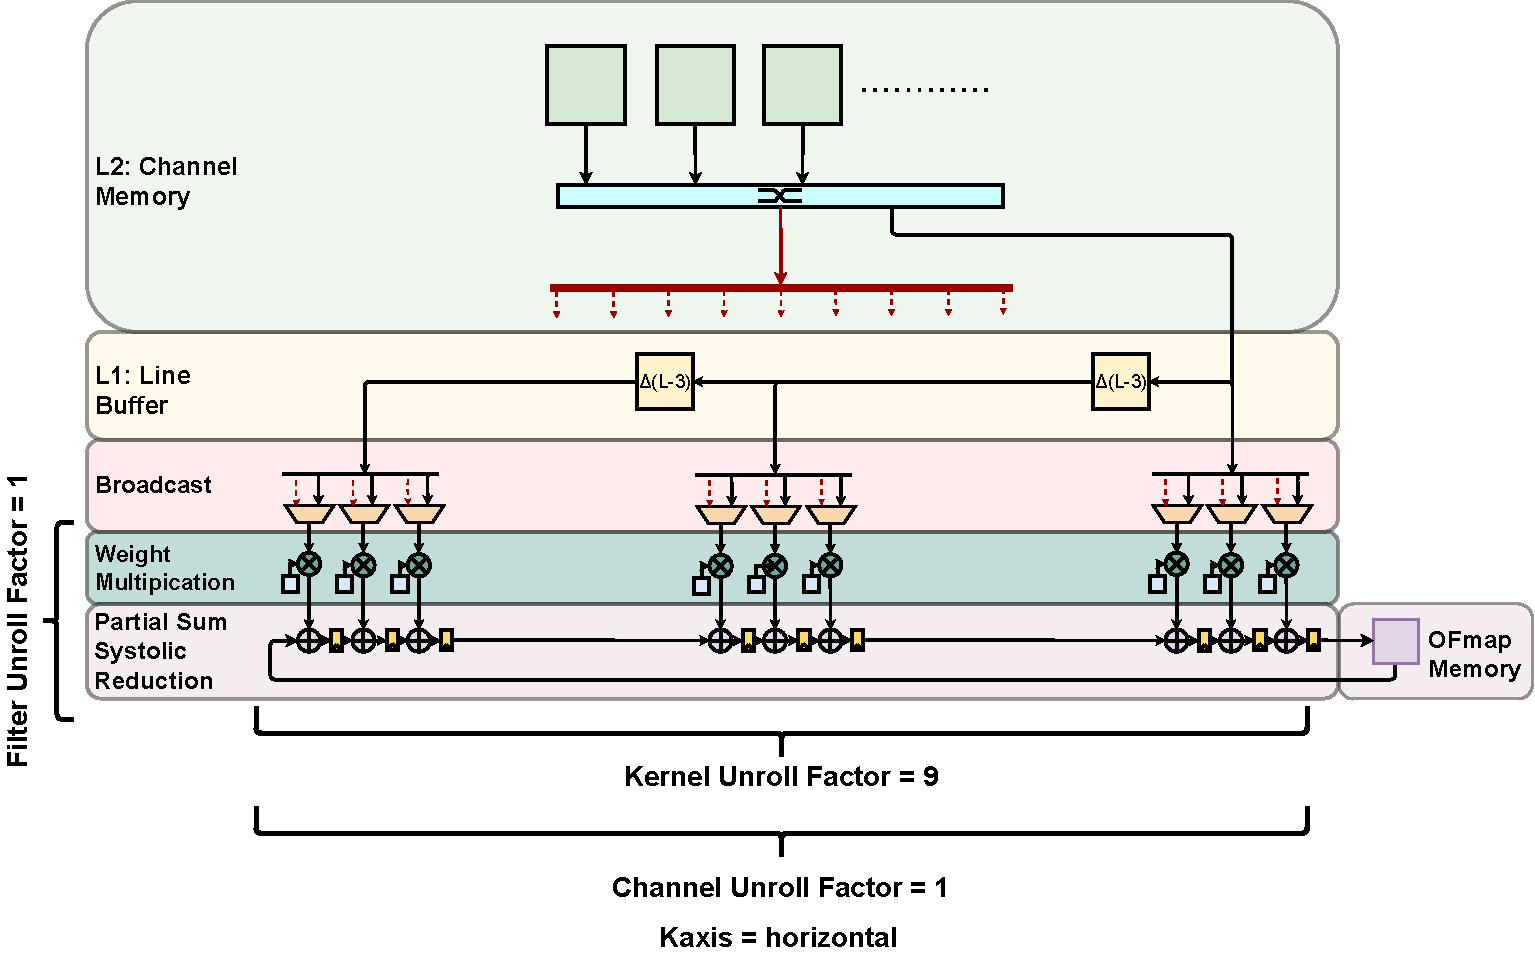
\includegraphics[scale=0.36]{fig/hybrid3x3Gemm.pdf}
    \caption{Using a systolic reduce and forward to calculate OFmaps}
    \label{fig:simplified_systolic_reduction}
\end{figure}

Substituting the InitialOffset function in $A_\Delta$  allows us to simplify the
column offset. This yields a new column offset $X'_i$. The final delayed access
function's initial offset becomes insensitive to changes in the port index $i$
that are not multiples of $K$. This allows us to remove the lowest layer memory
along with the systolic array delays in \autoref{fig:reuse_chain} and replace
both layers with just a series of broadcast buses that span consecutive $K$
groups of IFmap ports provided that we relax the start time constraints to the
$\lceil \frac{i}{K} \rceil$ for each group of ports $\lfloor \frac{i}{K}
\rfloor$. Delays in accessing IFmap data elements accross $K$ groups of ports
as well as accross $K^2$ groups of ports accessing different channels still
remain. This simplifying the hierarchy by removing the systolic delays thus still
requiring complex delayed reads from the IFmap hierarchy which necessitates smart
SRAMS whose access times can be programmed. A discussion of these smart memories
is presented in \autoref{chap:acc_sched:primitives:da-sram}. The final
hardware implementation with the added IFmap memory hierarchy optimization
discussed in this section is given in
\autoref{fig:simplified_systolic_reduction}.
\autoref{fig:simplified_systolic_reduction} shows the broadcast busses for every
group of 3 processing engines as well as the 1x1 vertical broadcast busses
highlighted in red. 


% https://www.desmos.com/calculator/y0oszemsuo

% Under 3x3/1x1 Direct Highest level ifmap. Layer size graph, ub 2\^19 bytes
% covers 95\% of networks. This leads to small area size (reference Jinghan paper)
% Does not scale with systolic array size. PSUM storage, depends on tiling
% schedule. Reference WC and psum storage scaling graph. WC equal to layer size
% graph ub. Scales with systolic array. Weights are reused then discarded for one
% inference pass. Double buffer and stream from memory. If model size is small
% enough/ sparsity is taken advantage of, we can store the weights on chip.
% However, this was not considered in this work. 

% GEMM mode im2col not only way of reshaping data. im2col maximizes bloat for
% ifmap. Solution is less bloaty im2col. Max storage required will be less 2\^19
% with balanced lifting and lowering. This implies that CPU has to do some vector
% ops concurrently with accelerator or vector ops should be added to accelerator.
% This not considered in this work.  

% moving on to memory scalability
% ifmap memory, we need 2\^19 bytes to support 95\% of networks
% layers that exceed that size are assumed to be too large
% we can trade off ifmap memory with psum memory if we switch loop ordering
% (show trade off graph), F, C is ASAP, C, F is alap. under asap
% psum storage scales with F, under alap max number of ofmaps are 
% in flight so that maximizes psum storage but we only need to keep 
% C worth of tiles in flight

% weight storage scales with the size of the systolic array

% GEMM_ID:=[F, C, Z] -> { S[f,c,z] : 0<=f<F and  0<=c<C and 0<=z<Z and f%4=0 and c%4=0};
% GEMM_IFMAP:=([F, C, Z, ci] -> {S[f,c,z] -> IF[c+ci][z]})*GEMM_ID;
% GEMM_IFMAP_REUSE:=(GEMM_IFMAP.(GEMM_IFMAP^-1))*(GEMM_ID<<GEMM_ID);
% GEMM_PSUM:=([F, C, Z, fi] -> {S[f,c,z] -> PS[f+fi][z]})*GEMM_ID;
% GEMM_PSUM_REUSE:=(GEMM_PSUM.(GEMM_PSUM^-1))*(GEMM_ID<<GEMM_ID);
% GEMM_WEIGHT:=([F, C, Z, fi, ci] -> {S[f,c,z] -> W[f+fi][c+ci]})*GEMM_ID;
% GEMM_WEIGHT_REUSE:=(GEMM_WEIGHT.(GEMM_WEIGHT^-1))*(GEMM_ID<<GEMM_ID);


% DIRECT_ID:=[F, C, Y, X] -> { S[f,c,y,x] : 0<=f<F and 0<=c<C and 0<=y<Yth
% and 0<=x<X and f%4=0 and c%4=0};
% DIRECT_IFMAP:=([F, C, Y, X, ci, ky, kx] -> {S[f,c,y,x] -> IF[c+ci][y+ky][x+kx]})*DIRECT_ID;
% DIRECT_IFMAP_REUSE:=(DIRECT_IFMAP.(DIRECT_IFMAP^-1))*(DIRECT_ID<<DIRECT_ID);
% DIRECT_PSUM:=([F, C, Y, X, fi] -> {S[f,c,y,x] -> PS[f+fi][y][x]})*DIRECT_ID;
% DIRECT_PSUM_REUSE:=(DIRECT_PSUM.(DIRECT_PSUM^-1))*(DIRECT_ID<<DIRECT_ID);
% DIRECT_WEIGHT:=([F, C, Y, X, fi, ci, ky, kx] -> {S[f,c,y,x] -> W[f+fi][c+ci][ky][kx]})*DIRECT_ID;
% DIRECT_WEIGHT_REUSE:=(DIRECT_WEIGHT.(DIRECT_WEIGHT^-1))*(DIRECT_ID<<DIRECT_ID);


% YX_ID:=[Y, X, KY, KX] -> { S[y, x, ky, kx] : 0<=y<Y and 0<=x<X and 0<=ky<KY and 0<=kx<KX};
% YX_IFMAP:=([Y, X, KY, KX] -> {S[y, x, ky, kx] -> IF[y+ky][x+kx]})*DIRECT_KERNEL_ID;
% YX_IFMAP_REUSE:=(DIRECT_KERNEL_IFMAP.(DIRECT_KERNEL_IFMAP^-1))*(DIRECT_KERNEL_ID<<DIRECT_KERNEL_ID);
% YX_PSUM:=([Y, X, KY, KX] -> {S[y, x, ky, kx] -> PS[y][x]})*DIRECT_KERNEL_ID;
% YX_PSUM_REUSE:=(DIRECT_KERNEL_PSUM.(DIRECT_KERNEL_PSUM^-1))*(DIRECT_KERNEL_ID<<DIRECT_KERNEL_ID);
% YX_WEIGHT:=([Y, X, KY, KX] -> {S[y, x, ky, kx] -> W[ky][kx]})*DIRECT_KERNEL_ID;
% YX_WEIGHT_REUSE:=(DIRECT_KERNEL_WEIGHT.(DIRECT_KERNEL_WEIGHT^-1))*(DIRECT_KERNEL_ID<<DIRECT_KERNEL_ID);

% Reuse w.r.t F and C loops


% RDIST_R10:=ub(card(((R10^-1).(ID<<=ID)*(ID<<=ID)^-1).A0));
% RDIST_R21:=ub(card(((R21^-1).(ID<<=ID)*(ID<<=ID)^-1).A1));
% RDIST_R32:=ub(card((*(ID<<=ID)^-1).A2));
% RDIST_R43:=ub(card(((R43^-1).(ID<<=ID)*(ID<<=ID)^-1).A3));
% RDIST_R54:=ub(card(((R54^-1).(ID<<=ID)*(ID<<=ID)^-1).A4));
% RDIST_R65:=ub(card(((R65^-1).(ID<<=ID)*(ID<<=ID)^-1).A5));
% RDIST_R76:=ub(card(((R76^-1).(ID<<=ID)*(ID<<=ID)^-1).A6));
% RDIST_R87:=ub(card(((R87^-1).(ID<<=ID)*(ID<<=ID)^-1).A7));


% R43;
% $4 := [IFMAP_Y, IFMAP_X] -> { 
%     S[y, x] -> S[y' = y, x' = 1 + x] : 
%         0 <= y <= -3 + IFMAP_Y and 0 <= x <= -4 + IFMAP_X 
% }
% R54;
% $5 := [IFMAP_Y, IFMAP_X] -> { 
%     S[y, x] -> S[y' = y, x' = 1 + x] : 
%         0 <= y <= -3 + IFMAP_Y and 0 <= x <= -4 + IFMAP_X 
% }
% R65;
% $6 := [IFMAP_Y, IFMAP_X] -> { 
%     S[y, x] -> S[y' = 1 + y, x' = -2 + x] : 
%         0 <= y <= -4 + IFMAP_Y and 2 <= x <= -3 + IFMAP_X 
% }
% R76;
% $7 := [IFMAP_Y, IFMAP_X] -> { 
%     S[y, x] -> S[y' = y, x' = 1 + x] : 
%         0 <= y <= -3 + IFMAP_Y and 0 <= x <= -4 + IFMAP_X 
% }

%     R10:=(lexmin ((A1.A0^-1)*(ID<<ID)));
%     R21:=(lexmin ((A2.A1^-1)*(ID<<ID)));
%     R32:=(lexmin ((A3.A2^-1)*(ID<<ID)));
%     R43:=(lexmin ((A4.A3^-1)*(ID<<ID)));
%     R54:=(lexmin ((A5.A4^-1)*(ID<<ID)));
%     R65:=(lexmin ((A6.A5^-1)*(ID<<ID)));
%     R76:=(lexmin ((A7.A6^-1)*(ID<<ID)));
%     R87:=(lexmin ((A8.A7^-1)*(ID<<ID)));

% ID:=[IFMAP_Y, IFMAP_X] -> {S[y,x]:y>=0 and x>=0 and y<=IFMAP_Y-3 and x<=IFMAP_X-3};
% A0:=[IFMAP_Y, IFMAP_X] -> {S[y,x]->A[y+0,x+0]}*ID;
% A1:=[IFMAP_Y, IFMAP_X] -> {S[y,x]->A[y+0,x+1]}*ID;
% A2:=[IFMAP_Y, IFMAP_X] -> {S[y,x]->A[y+0,x+2]}*ID;
% A3:=[IFMAP_Y, IFMAP_X] -> {S[y,x]->A[y+1,x+0]}*ID;
% A4:=[IFMAP_Y, IFMAP_X] -> {S[y,x]->A[y+1,x+1]}*ID;
% A5:=[IFMAP_Y, IFMAP_X] -> {S[y,x]->A[y+1,x+2]}*ID;
% A6:=[IFMAP_Y, IFMAP_X] -> {S[y,x]->A[y+2,x+0]}*ID;
% A7:=[IFMAP_Y, IFMAP_X] -> {S[y,x]->A[y+2,x+1]}*ID;
% A8:=[IFMAP_Y, IFMAP_X] -> {S[y,x]->A[y+2,x+2]}*ID;

% R10:=(lexmin ((A1.A0^-1)*(ID<<ID)));
% R21:=(lexmin ((A2.A1^-1)*(ID<<ID)));
% R32:=(lexmin ((A3.A2^-1)*(ID<<ID)));
% R43:=(lexmin ((A4.A3^-1)*(ID<<ID)));
% R54:=(lexmin ((A5.A4^-1)*(ID<<ID)));
% R65:=(lexmin ((A6.A5^-1)*(ID<<ID)));
% R76:=(lexmin ((A7.A6^-1)*(ID<<ID)));
% R87:=(lexmin ((A8.A7^-1)*(ID<<ID)));
